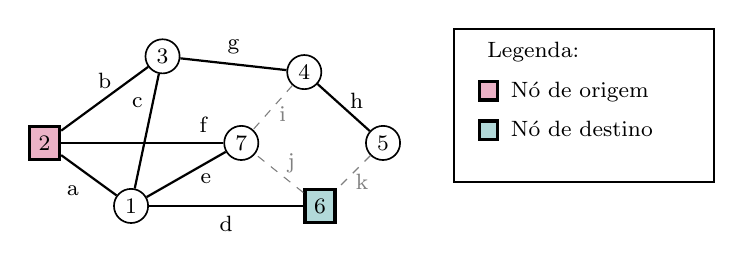
\begin{tikzpicture}
%============================================================
%  Essa seção define o estilo dos nós e arestas  
%  Necessário apenas para desenhar um grafo se quiserem
%============================================================
\tikzset{ % Importante:
          % Linha em branco nessa seção dá erro de compilação!
    % ESTILOS DOS GRAFOS
    % ---  Define arestas ------
    >=stealth,
    aresta/.style={ %
            -,     % sem terminação na aresta
            thick  % linha grossa
        },
    arco/.style={  % 
            ->,    % com seta no final da aresta
            thick  % linha grossa
        },
    outraAresta/.style={ -, %
            thin,  % linha fina
            dashed,% tracejada (dotted para pontilhada)
            gray   % cor da aresta 
        },
    % ---  Define vertices ------
    vertice/.style={   %
            circle,    % formato circular
            semithick, % linha "meio" grossa
            draw=black,% linha na cor preta
            inner sep=2pt % margem interna
        },
    verticeRetangular/.style={ %
            rectangle, % formato retangular
            very thick, % linha muito grossa
            draw=black  % linha na cor preta 
        },
    texto/.style={      %
            draw=white, % contorno em branco 
            font=\footnotesize %texto em letra pequena
        },
    % --- SOBRE CORES ------
    % Existem algumas cores padrão: blue, yellow, teal, 
    %     purple, red, violet, white, gray, lightgray...
    % As cores originais (principalmente blue, red, green)
    % são muito vivas, mas podem ser "diluidas": 
    %   blue!30         => 30% de azul com 70% de branco
    %   blue!80!black   => 80% de azul com 20% de preto
}


   % insere um nó com o estilo "vertice" (definido nas linhas 6 a 40 do arquivo)
   %    que será referenciado por v1 na posicao (x,y) do plano cartesiano indicada 
   %    com o texto interno "1"
   \node[vertice] (v1) at (0.6,0.2) {\footnotesize 1};
   % insere o vertice, mudando a cor padrão para 60% vinho 40% branco 
   % (veja comentario sobre cores nas linhas 40-46) 
   \node[verticeRetangular,fill=purple!30] (v2) at (-0.5,1) {\footnotesize 2};
   \node[vertice] (v3) at (1,2.1) {\footnotesize 3};
   \node[vertice] (v4) at (2.8,1.9) {\footnotesize 4};
   \node[vertice] (v5) at (3.8,1) {\footnotesize 5};
   \node[verticeRetangular,fill=teal!30] (v6) at (3,0.2) {\footnotesize 6};
   \node[vertice] (v7) at (2,1) {\footnotesize 7};


   
   % insere uma aresta com o estilo "aresta" (definido nas linhas 6 a 40)
   %    do nó v1 ao nó v2, com um nó intermediario contendo o texto "a"
   %    Os termos below, above, right, left, near start, near end ajudam a 
   %    posicionar o texto na aresta
   \draw[aresta] (v1) edge node[below left] {\footnotesize a} (v2);
   \draw[aresta] (v1) edge node[near end, left] {\footnotesize c} (v3);
   \draw[aresta] (v1) edge node[below] {\footnotesize d} (v6);
   \draw[aresta] (v1) edge node[near end, below] {\footnotesize e} (v7);
   \draw[aresta] (v2) edge node[above] {\footnotesize b} (v3);
   \draw[aresta] (v2) edge node[very near end, above] {\footnotesize f} (v7);
   \draw[aresta] (v3) edge node[above] {\footnotesize g} (v4);
   \draw[aresta] (v4) edge node[near end, above] {\footnotesize h} (v5);
   \draw[outraAresta] (v4) edge node[near start, below] {\footnotesize i} (v7);
   \draw[outraAresta] (v5) edge node[near start, below] {\footnotesize k} (v6);
   \draw[outraAresta] (v6) edge node[near start, above] {\footnotesize j} (v7);


    % Legenda 
    \node[texto,anchor=north west] (titulolegenda) at (5,2.4) {Legenda:};  
    \node[verticeRetangular,fill=purple!30,anchor=north west] (leg1) at (5,1.8) {};
    \node[texto,anchor=north west] (leg1txt) at (5.3,1.9) {Nó de origem};
    \node[verticeRetangular,fill=teal!30,anchor=north west] (leg1) at (5,1.3) {};
    \node[texto,anchor=north west] (leg1txt) at (5.3,1.4) {Nó de destino};
    
    \draw[aresta] (4.7,2.45) -- (8,2.45) -- (8,0.5) -- (4.7,0.5) -- cycle;
\end{tikzpicture}